\section{Generation Pipeline}
\label{sec:generation-pipeline}

Every sample is generated synthetically by prompting a large language model. The generation uses, for different tasks, Claude Haiku 4.5 and Claude Sonnet 5, both models provided by Anthropic. This section describes the stages that compose the generation pipeline, and discusses the sample count and distribution of the final single-turn and multi-turn datasets.

\subsection{Scenarios}
\label{subsec:scenarios}

Every request is grounded in a \textbf{scenario}: a short description of a software system under construction or under maintenance. The scenario set consists of 30 hand-authored scenarios. As the example below shows, a scenario describes only the system, with no sub-agent requests and no constraint, so a different binding constraint can be written for each of the five sub-agents from Section~\ref{subsec:sub-agent-taxonomy}, against the same scenario.

\begin{scenariobox}{Example -- scenario}
\textit{``An image processing routine converts every uploaded picture to a full-resolution intermediate representation in memory before applying any transformation.''}
\end{scenariobox}

\subsection{Facts}
\label{subsec:pipeline-facts}

For every scenario, a \textbf{fact} is generated for each sub-agent: one requirement on that system, owned by that sub-agent. The fact names the authority who imposes the requirement and what it demands. Each fact is generated with Claude Haiku 4.5. The example below shows two of the five facts drawn from the scenario in Section~\ref{subsec:scenarios}, one for \texttt{resource\_opt} and one for \texttt{legacy\_compat}.

\begin{scenariobox}{Example -- fact (\texttt{resource\_opt})}
\textit{``The cloud cost controller has capped monthly compute expenses at a fixed tier, which means the team must reduce the memory footprint of image processing by at least sixty percent from its current full-resolution approach to stay within budget without purchasing larger instances.''}
\end{scenariobox}

\begin{scenariobox}{Example -- fact (\texttt{legacy\_compat})}
\textit{``The published API contract guarantees that the image processing endpoint accepts files up to five gigabytes and returns the full intermediate representation upon request, so the team cannot change the in-memory storage behavior or response format without breaking existing client integrations.''}
\end{scenariobox}

\subsection{Sample Distribution}
\label{subsec:sample-distribution}

Generating one fact per sub-agent, for every scenario, yields 5 facts per scenario, 150 facts in total across the 30 scenarios. Since a request is generated from one or more facts, each stating one of its constraints, the number of available facts motivates the number of samples generated at each difficulty tier described in Section~\ref{subsec:difficulty-tiers}, and their distribution across sub-agents, reported in Table~\ref{tab:sample-distribution}.

\begin{table}[h]
    \centering
    \begin{tabular}{@{}lll@{}}
        \toprule
        \textbf{Tier} & \textbf{Per sub-agent} & \textbf{Total} \\
        \midrule
        \texttt{plain} & 30 & 150 \\
        \texttt{natural} & 120 & 600 \\
        \texttt{adversarial} & 180 & 900 \\
        \bottomrule
    \end{tabular}
    \caption[Sample counts per difficulty tier, single-turn and multi-turn]{Sample counts per difficulty tier, for each of the single-turn and multi-turn datasets.}
    \label{tab:sample-distribution}
\end{table}

The \texttt{plain} tier generates one request from each fact, stating that fact as the binding constraint. Every sub-agent owns 30 facts, one per scenario, so this gives 30 samples per sub-agent and 150 in total.

The \texttt{natural} tier generates one request from two facts, one for the binding constraint and one for the waived constraint. Swapping the two facts gives a different sample, since the binding fact sets the label. Every sub-agent is paired with each of its 4 colliding partners from Table~\ref{tab:collision-graph} in 30 samples, which gives 120 samples per sub-agent and 600 in total.

The \texttt{adversarial} tier builds pairs of requests instead of single requests: two facts are picked, and two requests are generated that share nearly all their wording, with a different one of the two facts stated as the binding constraint in each. The full design would pair every scenario with every one of the four decoy patterns from Section~\ref{subsec:difficulty-tiers}, for every colliding pair of sub-agents, and generate two requests per pairing. This would yield 2400 samples. Fewer are generated: 900 in total, 180 per sub-agent. This choice follows from budget: adversarial pairs are the most expensive samples to generate. The adversarial tier is set to 1.5 times the natural tier, so that the hardest tier is the largest in the dataset. Section~\ref{sec:dataset-baselines} confirms that the reduced number of adversarial samples does not affect the quality of the result.

\subsection{Plan}
\label{subsec:pipeline-plan}

The \textbf{plan} stage takes the sample counts fixed in Section~\ref{subsec:sample-distribution} and scaffolds every sample in the dataset. For each sample, it sets:

\begin{itemize}
    \item the sub-agent the sample must route to;
    \item the scenario it draws from and, within it, the fact that states this sub-agent's binding constraint;
    \item at the \texttt{natural} tier, the colliding sub-agent and the fact that defines its waived constraint;
    \item at the \texttt{adversarial} tier, the decoy sub-agent, the fact that defines its waived constraint, and the decoy pattern used to write it;
    \item the persona from Section~\ref{subsec:personas} that writes the request.
\end{itemize}

Every sub-agent has the same number of samples. Each scenario, persona, and decoy pattern also appears in the same number of samples for every sub-agent. This is the balance requirement that Section~\ref{subsec:lexical-separability} demands: without it, a sub-agent could be told apart by its sample count, its scenarios, or its writing style rather than by the constraint it owns. The scenarios, personas, decoys, and decoy patterns assigned to a sub-agent are shuffled separately, so that no scenario is always paired with the same persona, decoy, or decoy pattern.

The shuffle uses a fixed random seed, so it is deterministic: every run of the plan stage produces the same plan. Because the plan fixes every sample's design before any request is generated, the generation stage can be re-run multiple times, and each run generates only the samples that are still missing. This allows the dataset to be generated in parts instead of all at once, so that each part can be reviewed before the next one is generated. It also allows targeted regeneration: only the samples flagged by the audit stage (Section~\ref{subsec:pipeline-audit-repair}) are generated again.

\subsection{Generate}
\label{subsec:pipeline-generate}

The \textbf{generate} stage prompts a large language model for each sample, using the sample configuration the plan stage determined. The prompt asks for the text of the user message, or, for a multi-turn sample, the full conversation. Appendix~\ref{chap:appendix-prompts} reports all the prompts used.

The \texttt{plain} prompt instructs the model to treat one fact as the binding constraint. The \texttt{natural} prompt provides two facts and instructs the model to treat one as binding and the other as waived. The \texttt{adversarial} prompt provides two facts and the decoy pattern that the plan stage assigned. It instructs the model to write a pair of requests at once, following that pattern, so that the two requests share nearly all their wording and differ only in which fact is stated as binding. A multi-turn sample uses a separate prompt from its single-turn counterpart at the same tier, since it must render a conversation instead of one request.

An \texttt{adversarial} pair is generated in a single call, as one contrastive unit: the model is asked for both members of the pair together, so it keeps their shared wording close, instead of generating each member separately and risking a pair that does not overlap enough. For multi-turn samples, the two members of a pair share every turn up to, but not including, the last one: only the last turn differs between them, and it is this turn that carries the binding constraint.

Claude Haiku 4.5 was used to generate every request, except the multi-turn \texttt{adversarial} ones. For these, the audit stage (Section~\ref{subsec:pipeline-audit-repair}) flagged a large share of the samples generated with Claude Haiku 4.5. Manual inspection of the flagged samples, and repeated generation attempts, showed that the model could not reliably follow the constraints stated in its prompt for these requests, so Claude Sonnet 5 was used in its place.

\subsection{Audit and Repair}
\label{subsec:pipeline-audit-repair}

Once generation is complete, a set of checks is applied to every sample.

\paragraph{Structural Checks.} A request is checked against a length range, to catch a malformed generation, such as text cut short mid-sentence. A multi-turn sample is also checked to ensure that the turn alternation and the number of turns are correct, and every sample is checked for text that names one of the sub-agents directly, since a request that names its target gives the label away rather than letting it follow from the constraint.

\paragraph{Jaccard Index.} For an \texttt{adversarial} pair, the two members are checked for how much their words overlap. The check uses the Jaccard index \cite{nobleWhatJaccardSimilarity2026}, computed on the word sets $A$ and $B$ of the text that decides the label, for each of the two members:
\begin{equation}
    J(A, B) = \frac{|A \cap B|}{|A \cup B|}
\end{equation}
For a multi-turn pair, only the last user message is used, since Section~\ref{subsec:multiturn-derivation} makes it the only message that can differ between the two members. A pair whose two members share little wording is not contrastive: the label could be read off the surrounding text rather than the pivot that the pair is built around. The floor was set to 0.60 after a manual review of a subset of pairs. A pair whose Jaccard index falls below 0.60 is dropped, and the sample needs to be regenerated.

\paragraph{Oracle Check.} Claude Sonnet 5 is invoked as an oracle, for each generated request. It reads the request, with no view of the plan's intended sub-agent, and decides on its own which constraint is binding and which sub-agent owns it. This verdict, and the quote it is based on, are written back onto the sample and checked against the plan's intended sub-agent. The check confirms that the request carries enough information to route it to exactly one sub-agent, the requirement that Section~\ref{sec:dataset-requirements} states. A sample that the oracle flags, either because it disagrees with the plan or because it cannot decide, requires manual revision: it can be corrected by hand, marked as correct despite the oracle's verdict, or dropped so it can be regenerated.

A separate \texttt{repair} stage acts on the \texttt{regenerate} flag these checks set, whether from a failed check or from manual revision. It deletes every sample still carrying the flag, so the next \texttt{generate} run recreates it from the same plan row, without touching the plan or the samples that the checks did not flag. An \texttt{adversarial} pair is always regenerated as a whole: if one member is dropped, both are deleted and regenerated together, since a repaired half-pair could no longer be guaranteed to overlap with its twin the way that the Jaccard index check requires.

Figure~\ref{fig:pipeline-stages} shows the complete pipeline, from the scenario set to a checked sample, and the loop that a failed sample takes back to \texttt{generate}.

\begin{figure}[h]
    \centering
    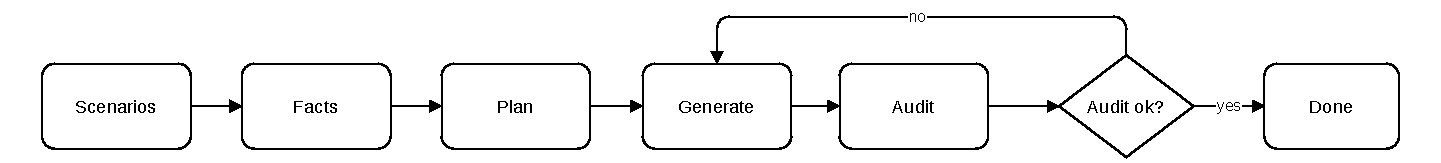
\includegraphics[width=\textwidth]{images/generation_pipeline.pdf}
    \caption[Generation pipeline, sample regenerated on audit failure]{The generation pipeline. A sample that fails the audit stage is regenerated.}
    \label{fig:pipeline-stages}
\end{figure}

\subsection{Cost}
\label{subsec:pipeline-cost}

Table~\ref{tab:pipeline-cost} reports the cost of producing both datasets, at Claude's Batch API prices, which halve the standard per-token rate. Each stage's figure is the total cost across every \texttt{generate} and \texttt{audit} iteration needed to reach the final set of samples, rather than the cost of a single pass. The \texttt{plan} and \texttt{facts} stages are not included: \texttt{plan} calls no model, and \texttt{facts} generates 150 short requests in total, a negligible cost next to the other stages.

\begin{table}[H]
    \centering
    \small
    \setlength{\tabcolsep}{3.5pt}
    \begin{tabular}{@{}llrrrrr@{}}
        \toprule
        & & \multicolumn{4}{c}{\textbf{Tokens (millions)}} & \\
        \cmidrule(lr){3-6}
        \textbf{Stage} & \textbf{Model} & \textbf{Input} & \textbf{Output} & \textbf{Cache read} & \textbf{Cache write} & \textbf{Cost} \\
        \midrule
        \texttt{generate}, single-turn            & Claude Haiku 4.5 & 4.32 & 0.61 & 0.00 & 0.00 & \$3.68 \\
        \texttt{generate}, multi-turn              & Claude Haiku 4.5 & 2.02 & 0.45 & 0.00 & 0.00 & \$2.15 \\
        \texttt{generate}, multi-turn \texttt{adversarial} & Claude Sonnet 5  & 1.49 & 1.44 & 1.40 & 2.34 & \$8.68 \\
        \texttt{audit}, single-turn                & Claude Sonnet 5  & 1.27 & 0.50 & 4.37 & 1.24 & \$3.78 \\
        \texttt{audit}, multi-turn                 & Claude Sonnet 5  & 2.38 & 0.53 & 4.77 & 1.23 & \$5.01 \\
        \midrule
        \textbf{Total} & & \textbf{11.47} & \textbf{3.53} & \textbf{10.54} & \textbf{4.81} & \textbf{\$23.30} \\
        \bottomrule
    \end{tabular}
    \caption[Tokens and cost for the single-turn and multi-turn datasets]{Tokens and cost of the run that produced the single-turn and multi-turn datasets, at Claude's Batch API prices. Input counts only the uncached input tokens.}
    \label{tab:pipeline-cost}
\end{table}
